\section{Calculs de statique et de dynamique}
\label{meca}
Le but est de déterminer une vitesse max en virage sans renversement du chariot; et une vitesse max en ligne droite garantissant une décélération sans glissement du colis.

Pour cela, nous utiliserons des équations de dynamique, ce qui suppose de modéliser le chariot. Nous ferons donc des hypothèses sur sa forme géométrique et la répartition de sa masse. Ensuite, nous avons obtiendrons par des théorèmes les équations attendues: vitesse max en ligne droite, vitesse max en virage. Enfin, nous vérifierons l'adéquation de ces résultats avec des mesures sur un modèle physique de chariot que nous avons construit (nous l'appelerons le prototype).

\label{hypProtoCommeChariot}
Mais la validation des hypothèses sur le chariot élévateur par des mesures sur notre prototype mécanique nécessite de supposer que notre prototype mécanique est lui-même un bon modèle qui se comporte comme un chariot élévateur. Elle permet en fait de généraliser l'ensemble des productions de notre TX (modèles mécaniques et numériques, voir \ref{proto}) à tous les chariots élévateurs, et à tous les véhicules verticaux, fins et avec un centre de masse haut. Elle pourrait être appuyée par des arguments théoriques, mais le seul argument que nous fournirons est le fait que toutes les dimensions sont du même ordre de grandeur. Cette hypothèse est très forte, mais elle n'est pas critique: si elle n'était pas vraie, cela signifierait que nos productions ne seraient valables que pour notre prototype.

\subsection{Description de l'étude}
Le cadre qu'on s'est fixé pour cette étude est fortement inspiré de \cite{arnaud}.
\begin{itemize}
	\item Le hangar est muni du repère $R_g = (O,\vec x_g, \vec y_g, \vec z_g)$.
	\item Le chariot $(0)$ est animé d'un mouvement de rotation par rapport au sol dont le centre instantané de rotation est $O$.
	\item Le rayon de courbure de la trajectoire du point C dans $R_g$ est $R$.
	\item Le repère lié à $(0)$ est $R_0 = (O, \vec x_0, \vec y_0, \vec z_0)$ tel que $\vec z_0 = \vec z_g$ et on note $\theta = (\vec x_g, \vec x_0) = (\vec y_g, \vec y_0)$.
	\item Donc $\vec{OC} = R \cdot \vec x_0$. On remarque bien que $R_0$ est mobile par rapport à $R_g$.
	\item On considère que les frottements du colis $(1)$ l'encastrent avec le chariot $(0)$.
	\item Le repère lié au colis est $R_1 = (C, \vec x_1, \vec y_1, \vec z_1)$ et tant qu'il n'y a pas glissement du colis, $\vec e_1 = \vec e_0 \forall e \in \{x,y,z\}$.
	\item Le centre de gravité du colis est $G$ tel que $\vec{CG} = e\cdot\vec z_1$. La masse du colis est m.
		\begin{itemize}
			\item On donne son opérateur d'inertie en G:$\overline{\overline{I}}_A(1) = \left[ \begin{array}{ccc}
					A & -F & -E \\
					-F & B & -D \\
					-E & -D & C
			\end{array} \right]_{B0}$
		\end{itemize}
	\item Les roues arrière $(2)$ et $(3)$ sont liées à $(0)$ par des liaisons pivots d'axe $(C, \vec x_0)$.
	\item Les contacts entre les roues $(2)$ et $(3)$ et le hangar $(R)$ ont lieu en $A$ et $B$ définis par $\vec{CA} = \frac{l}{2} \cdot \vec x_0 - r\cdot \vec z_0$ et $\vec{CB} = -\frac{l}{2} \cdot \vec x_0 - r\cdot \vec z_0$, $r$ désignant le rayon des roues et $l$ la voie arrière du chariot.
	\item Les contacts sont modélisés par des liaisons sphère-plan de centres $A$ et $B$ et de normale $\vec z_0$.
	\item Le contact dans ces liaisons se fait avec frottement et le coefficient de frottement est noté $f$ (on supposera pour simplifier que les coefficients de frottement et d'adhérence sont identiques).
	\item Les actions mécaniques du hangar $(R)$ sur les roues $(2)$ et $(3)$ sont modélisées dans le plan $(\vec x_0, \vec y_0)$ par des glisseurs en $A$ et $B$ de résultantes: \[
			F(R\rightarrow 2) = T_A\cdot \vec x_0 + N_A \cdot \vec z_0 \text{ et } F(R\rightarrow 3) = T_B\cdot \vec x_0 + N_B\cdot z_0 \]
	\item A part les liaisons entre $(R)$ et $(2)$ et entre $(R)$ et $(3)$, pour lesquelles le frottement est pris en compte, toutes les liaisons sont considérées parfaites.
	\item On néglige la masse et l'inertie de $(0)$, $(2)$ et $(3)$ devant celle du colis $(1)$. On note $E = 0 \cup 1 \cup 2 \cup 3$. L'accélération de la pesanteur est $\vec g = -g \cdot \vec z_0$.
	\item On se place dans un cas où le rayon de courbure $R_C$ de la trajectoire du point C, ainsi que la vitesse V de ce point par rapport au référentiel $R_g$ sont constants.
	\item Le contact entre le colis et le chariot est modélisé par une liaison plan à plan, avec un coefficient de frottement $\mu$.
\end{itemize}
\begin{figure}
	\centering
	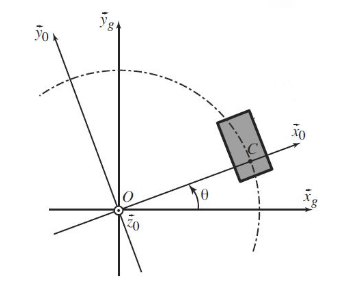
\includegraphics[height=5cm]{schema_chariot3}
	\caption{Le virage du chariot paramétré}
	\label{fig:schemaChariot3}
\end{figure}
\subsection{Calculs}
\paragraph{Vitesse de $G$ dans $R_g$}
\[\vec{OG} = \vec{OC} + \vec{CG} = R_c \cdot \vec x_0 + e\cdot \vec z_1 = R_c \cdot \vec x_0\]
\[\vec V(G/R_g) = \frac{d\vec{CG}}{d_t}_{R_g} = \dot \theta \vec z_0 \wedge R_c \dot \theta \vec y_0 = -R_c \dot \theta^2 \vec x_0 \]
Avec $ V = R_c \dot \theta$ on obtient:
\begin{equation}
	\vec V(G / R_g) =V \vec y_0
\end{equation}
\paragraph{Accélération de $G$ dans $R_g$}
\[\vec a(G/R_g) = \frac{d}{dt}\vec V(G/R_g)_{R_g} = \dot \theta \vec z_0 \wedge R_c \dot \theta \vec y_0 = - R_c \dot \theta^2 \vec x_0\]
Avec $V=R_c \dot \theta$ on obtient:
\begin{equation}
	\vec a(G/R_g) = - \frac{V^2}{R_c} \vec x_0
\end{equation}
\paragraph{Moment dynamique en G de E dans son mouvement par rapport à $R_g$}
\[ \vec \delta (G, E / R_g) = \frac{d}{dt} \vec \sigma (G, E/R_g)_{R_g} = \frac{d}{dt} \left( I(G,E) \cdot \vec \Omega (E / R_g) \right)_{R_g} = \frac{d}{dt} \left( - E \dot \theta \vec x_0 - D \dot \theta \vec y_0 + C \dot \theta \vec z_0 \right)_{R_g} \]
Soit
\begin{equation}
	\vec \delta (G, E/R_g) = -E \dot \theta^2 \vec y_0 + D \dot \theta^2 \vec x_0
\end{equation}
\paragraph{Actions mécaniques de contact entre le hangar et les roues}
\[
	\text{TRD :} \vec F (R \rightarrow 2) + \vec F (R \rightarrow 3) + \vec F(\text{pes} \rightarrow E) = m\cdot \vec a(G/R_g)
\]
Soit:
\begin{equation}
	T_A + T_B = -m \frac{V^2}{R_c}
\end{equation}
et
\begin{equation}
	N_A + N_B - m\cdot g = 0
\end{equation}
\[
	\text{TMD: } \vec M(B,R \rightarrow 2) + \vec M(B,R \rightarrow 3) + \vec M(B, \text{pes} \rightarrow E) = \vec \delta(B,E / R_g)
\]

\[
	\vec M(B,R \rightarrow 2) = B\vec A \wedge \vec F (R \rightarrow 2) = l \vec x_0 \wedge (T_A \vec x_0 + N_A \vec z_0) = -l\cdot N_A \cdot \vec y_0
\]
\[
	\vec M(B, pes \rightarrow E) = B \vec G \wedge -mg\vec z_0 = (\frac{l}{2}\vec x_0 + r\vec z_0 + e \vec z_1)\wedge -mg\vec z_0 = \frac{l}{2}mg\vec y_0
\]
\[
	\vec \delta(B, E/R_g) = \vec \delta(G, E/R_g) + B\vec G \wedge m \vec a(G/R_g) = (\frac{l}{2}\vec x_0 + r\vec z_0 + e\vec z_1) \wedge -m \frac{V^2}{R_c} \vec x_0
\]
\[
	\vec \delta(B,E/R_g) = -E \dot \theta^2 \cdot \vec y_0 + D \dot \theta^2 \cdot \vec x_0 - m(r+e)R_c\vec y_0
\]
Sur $\vec y_0$:
\begin{equation}
	-LN_A + \frac{l}{2}mg = -E \dot \theta^2 - m(r+e)\frac{V^2}{R_c}
\end{equation}
\paragraph{Efforts normaux $N_A$ et $N_B$ (en fonction de $m$, $l$, $r$, $e$, $g$, $R_c$ et $V$)}
En négligeant $E\dot\theta^2$ :
\begin{equation}
	N_A = m(r+e)\frac{V^2}{l\cdot R_C} + \frac{1}{2}mg
\end{equation}
\begin{equation}
	N_B = -m(r+e)\frac{V^2}{l\cdot R_C} + \frac{1}{2}mg
\end{equation}
Hypothèses : $e<R_c$ et $e<\frac{l}{2}$

Il y a décollement si l'effort normal devient négatif:
\begin{itemize}
	\item $N_A<0$ impossible, donc la roue extérieure reste en contact avec le hangar
	\item $N_B<0$ possible pour V assez grand
\end{itemize}
\paragraph{Condition de non-renversement}
Non décollement si $N_B>0$ implique $-m(r+e)\frac{V^2}{l\cdot R_c} > -\frac{1}{2}mg$
\begin{empheq}[box=\fbox]{equation}
	\frac{V^2}{R_c} < \left( \frac{l}{2(r+e)} \right) \cdot g
\end{empheq}
\paragraph{Condition d'adhérence}
Adhérence si $\left| \frac{T_A}{N_A} \right| < f$ et $\left| \frac{T_B}{N_B} \right | < f$, la tendance au glissement est suivant $\vec x_0$ donc $T_A$ et $N_A$ sont de même signe soit:
\[ |T_A + T_B| < f(N_A + N_B) \]
\[ T_A + T_B = -m \frac{V^2}{R_c} \]
et \[N_A + N_B - mg = 0\]
Soit \[ m \frac{V^2}{R_c} < f \cdot mg \]
\begin{empheq}[box=\fbox]{equation}
	\frac{V^2}{R_c} < f\cdot g
\end{empheq}
\subsection{Autres résultats et bilan}
On a maintenant deux équations qui nous permettent de connaître la vitesse max qu'on pourra avoir sur une trajectoire.

On peut aussi montrer que la durée minimale de parcours d'un virage est $t_1 = \pi\sqrt{\frac{R_c(r+e)}{2lg}}$, et que la durée minimale de parcours d'un couloir est $t_2=2\sqrt{\frac{l}{fg}}$.
